\chapter{Mechanical Design}

\graphicspath{{./Figures/Mechanical Design/}}




%	\item Outline the purpose and scope of the chapter.

 Modeling In this chapter, the details of the mechanical design are presented. where it goes from the initial conceptual design to the final design showing in the process the design decision-making for each critical point, This chapter emphasis the detailed description of the precise placement and alignment of different components such as the motors, wheels, battery, boards, and others to maintain the seamless integration of all the components into the robot body.
%	\item Briefly describe the mechanical design's role in the overall project.
\newline
The mechanical design serves as an important pillar to define the new physical form, size, and shape of the TWIPR. Depending on how these criteria are defined, the robot would interact with the environment. taking into account that the design directly influences the center of gravity, which is crucial to consider in our robot due to the inverted pendulum nature to be able to balance and maintain the upright position. In addition to the impact that the design has on the maneuverability of the robot and how it would respond to the control signals to be able to execute a task.

\newpage


\section{Design Objectives and Requirements}

%	Detail the primary objectives of the mechanical design
	The main objective is to come up with a new design for a multiple joints Robot to perform complex dynamic movements. this robot would be based on the Two wheeled inverted pendulum robot. The new design would add more degrees of freedom to enable the more complex movements.This enhances the robot capabilities where it can execute more diverse scenarios.
%	\item List the requirements that the design must meet (e.g., weight limits, size constraints, mobility requirements).
	Initially, the main requirement was to add two more degrees of freedom where originally it used to have one degree of freedom in the wheels. The new design has three degrees of freedom one in the wheels, one as a knee joint and one as a hip joint. The current design has two identical legs.

\section{Conceptual Design}
%Discuss the initial design concepts.
As for the initial design concepts the body was that main point of focus as shown in the figure \ref{fig:initialdesigns}.Three initial designs where considered mainly for the body.\ Symmetrical vertical body in figure A, symmetrical horizontal body in figure B and leaning forward body in figure C.
\ For the three designs, two independent legs where considered.
two designs where considered for the legs, the normal joint leg and the compliant leg

\begin{figure}[h]
	\centering
	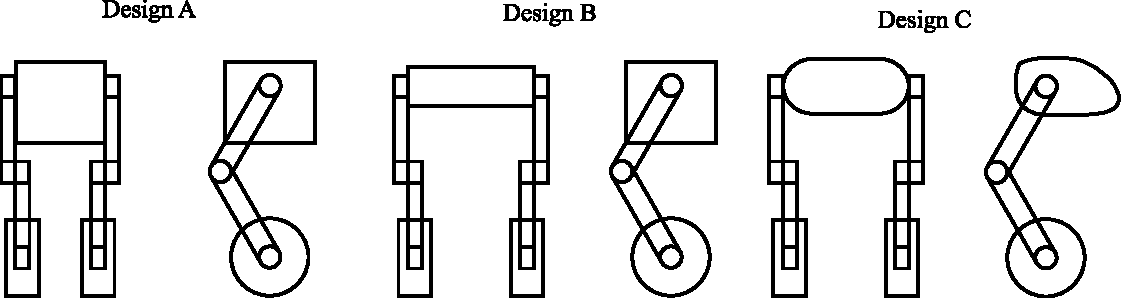
\includegraphics[width=1\linewidth]{Conceptual Design}
	%\includegraphics[width=0.5\linewidth]{Figures/Mechanical Design/Conceptual_Design}
	\caption[Initial Design Concepts TEST]{Three initial Design Concepts for the robot body}
	\label{fig:initialdesigns}
\end{figure}


Two main designs where considered for the legs, the normal joint leg and the compliant leg. The compliant leg is more flexible and can be used to absorb the shock from the ground.\ The normal joint leg is more rigid and can be used to generate more torque.in addition, the normal is more relative to our use-case as it can precisely control the position of the leg.


% figure for the leg designs
\begin{figure}[h]
	\centering
	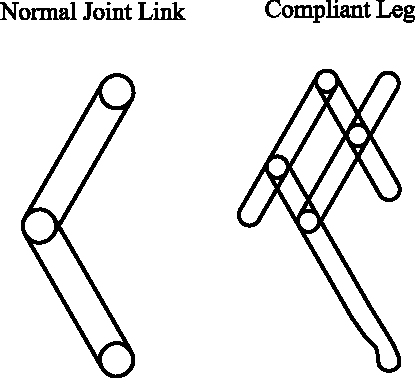
\includegraphics[width=0.4\linewidth]{Leg Design}
	\caption[between brakets for leg design]{Leg different Designs }
	\label{fig:legdesignsjbhi}
\end{figure}




%Explain the decision-making process for selecting the final concept.
% Include sketches or early design models.
\section{Initial Calculations}
%figure for the initial calculations
\begin{figure}[h]
	\centering
	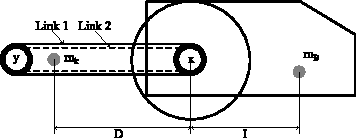
\includegraphics[width=0.7\linewidth]{Initial Calculations}
	\caption[Initial Calculations]{Initial Calculations}
	\label{fig:initialcalculations}
\end{figure}
One of the main critical positions for the robot, as shown in the figure \ref{fig:initialcalculations} is the position where the center of mass of the body and the center of mass of the legs are the furthest away from point x on the horizontal axis.It is important to make the initial torque calculations to be able to select the right motors for the robot.
Starting from that position first, the robot should be able to balance itself and maintain the upright position.
secondly, the robot should be able to change the knee angle to lift the body while maintaining its balance.
The calculations are based on some assumptions and simplifications, Considering only half the body weight and one leg joint.
As shown in the figure, The Wheel motor shaft is aligned with the hip joint, the minimum torque required to balance the robot is calculated as follows:

The summation of the torques around point x should be equal to zero to maintain the balance with minimum motor torque.
\begin{equation}
	\sum_{i=1}^{n} \tau_{i}=0
\end{equation}
\begin{equation}
	\sum_{i=1}^{n} \tau_{i}=m_{B}*g*D-m_{K}*g*I
\end{equation}
\begin{equation}
	\sum_{i=1}^{n} \tau_{i}=0.5*9.81*0.03-0.2*9.81*0.5*0.15=0 Nm
\end{equation}
The Lengths of D and I can be modified to make sure that the summation of the torques around point x is equal or approximately equal to zero.
This will make sure that the robot can balance itself with minimum wheel motor torque.
The torque required to lift the body is calculated as follows:
\begin{equation}
	\sum_{i=1}^{n} \tau_{i}=m_{B}*g*(D+I)-m_{K}*g*L_{1}
\end{equation}
\begin{equation}
	\sum_{i=1}^{n} \tau_{i}=0.5*9.81*(0.03+0.15)-0.1*9.81*0.5*0.15=0.9555 Nm
\end{equation}
0.9555 Nm is the minimum torque required to hold the body in position.
The motor should be able to generate more torque to be able to lift the body and change the knee angle.

table for the assumptions
\begin{table}[h]
	\centering
	\caption{Assumptions}
	\label{tab:assumptions}
	\begin{tabular}{lcl}
		\toprule
		Parameter & Value & Description 			  \\
		\midrule
		$m_B$         & 0.5 kg  & Mass of the body  \\
		$m_K$         & 0.2 kg  & Mass of the Knee including the two legs\\
		$L_1$         & 0.15 m   & Length of Link 1  \\
		$L_2$         & 0.15 m   & Length of Link 2   \\
		$d$ 	  	  & 0.3 m   & distance from the hip joint axis to the center of mass of the body   \\
		\bottomrule
	\end{tabular}
\end{table}

\begin{notebox}
	\textbf{To reduce the needed torque to lift we can:}
	%bullit points
	\begin{itemize}
		\item shorten the links then calculate position 4 again
		\item reduce the body weight then calculate position 4 again
		\item use gearbox then calculate position for again
	\end{itemize}
\end{notebox}
\section{Detailed Design Development}
% Elaborate on the development of the detailed mechanical design.

\subsection{Body Design}
% Discuss the design of the body.

\begin{figure}[h]
	\centering
	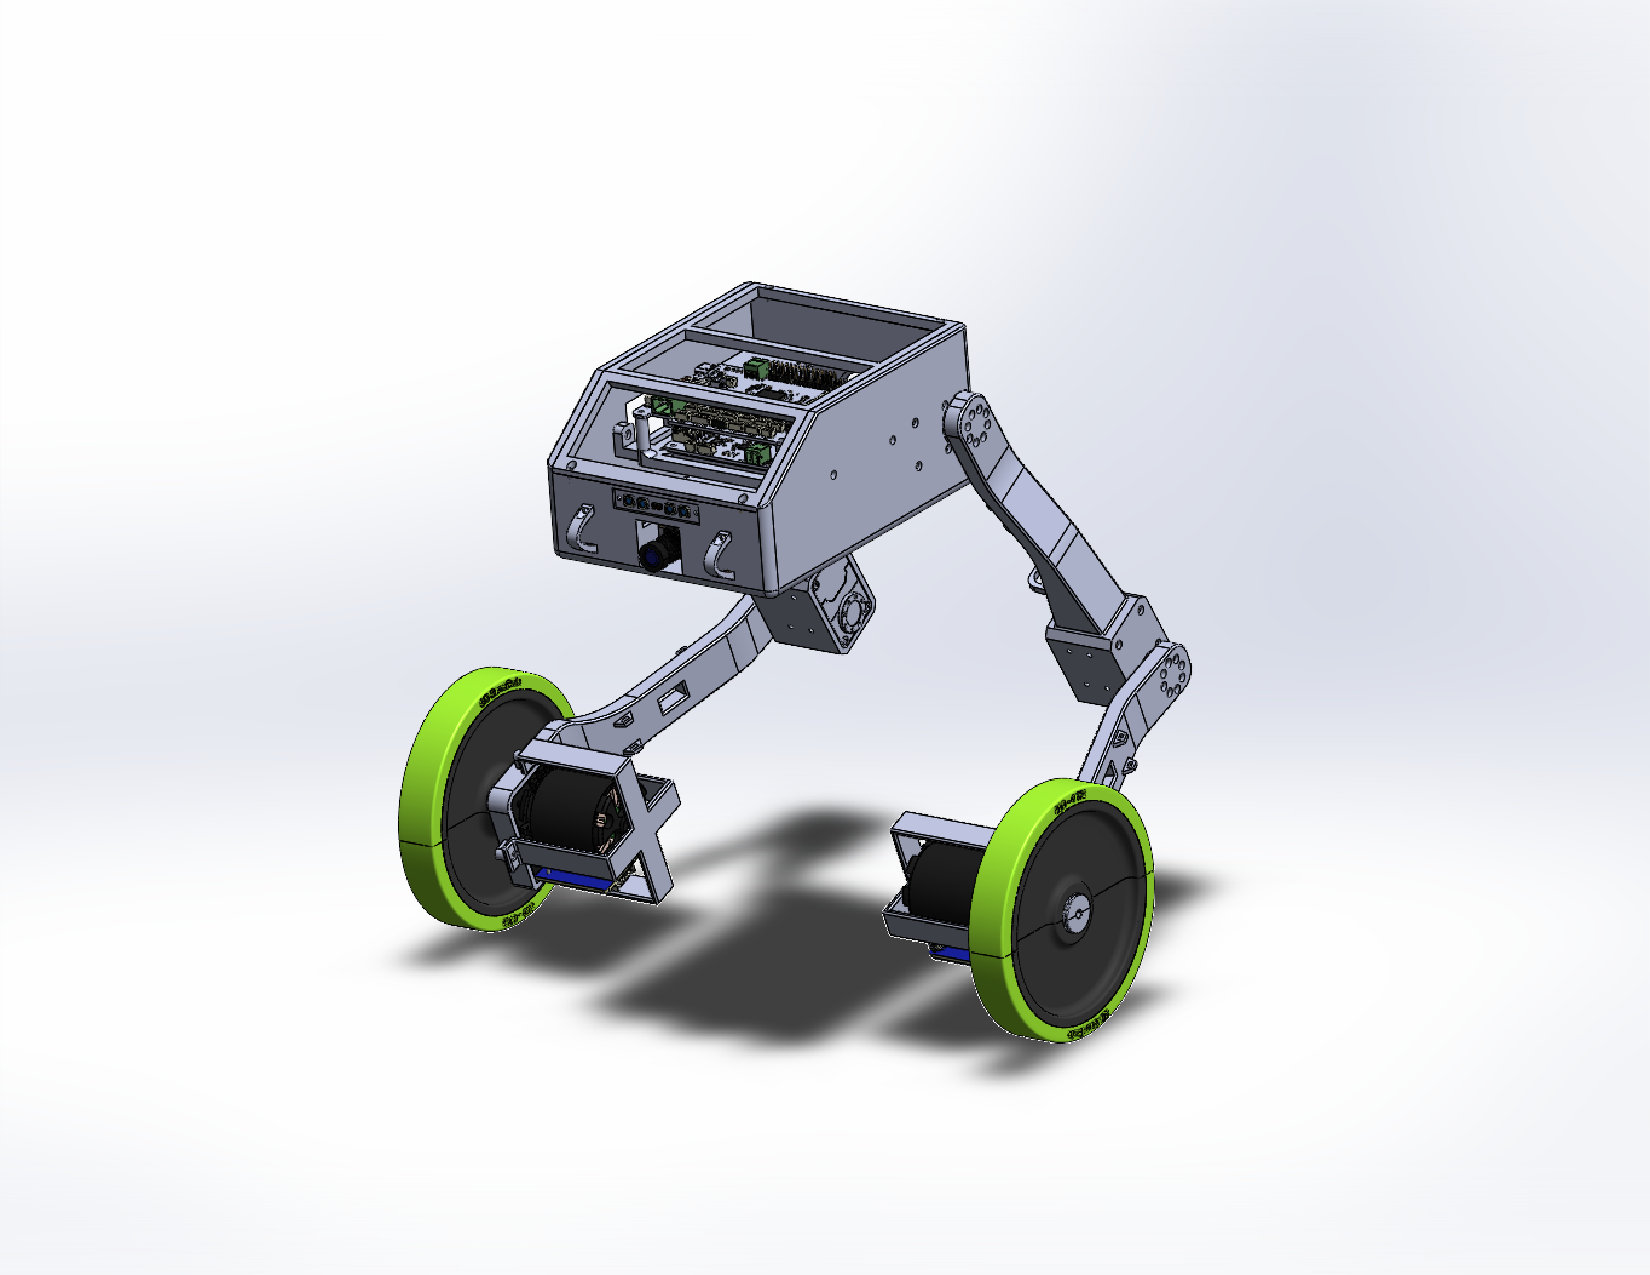
\includegraphics[width=0.7\linewidth]{Robot_Assembly_V2}
	\caption[Body Design]{Body Design}
	\label{fig:bodydesign}
\end{figure}

The body design is the main part of the robot, it is the main structure that holds all the components together.
% Discuss material selection and the rationale behind these choices.
% Include detailed CAD drawings and design schematics.



%This comprehensive chapter unfolds the intricate details of the new design of our two-wheeled self-balancing robot, an advanced piece of engineering that incorporates additional degrees of freedom to enhance its movement capabilities. Through an exploration of the various motions the robot can perform, we delve into the intricate design considerations of each component, ensuring that they align with the overall functional and aesthetic vision.
%
%
%\begin{figure}[h]
%	\centering
%	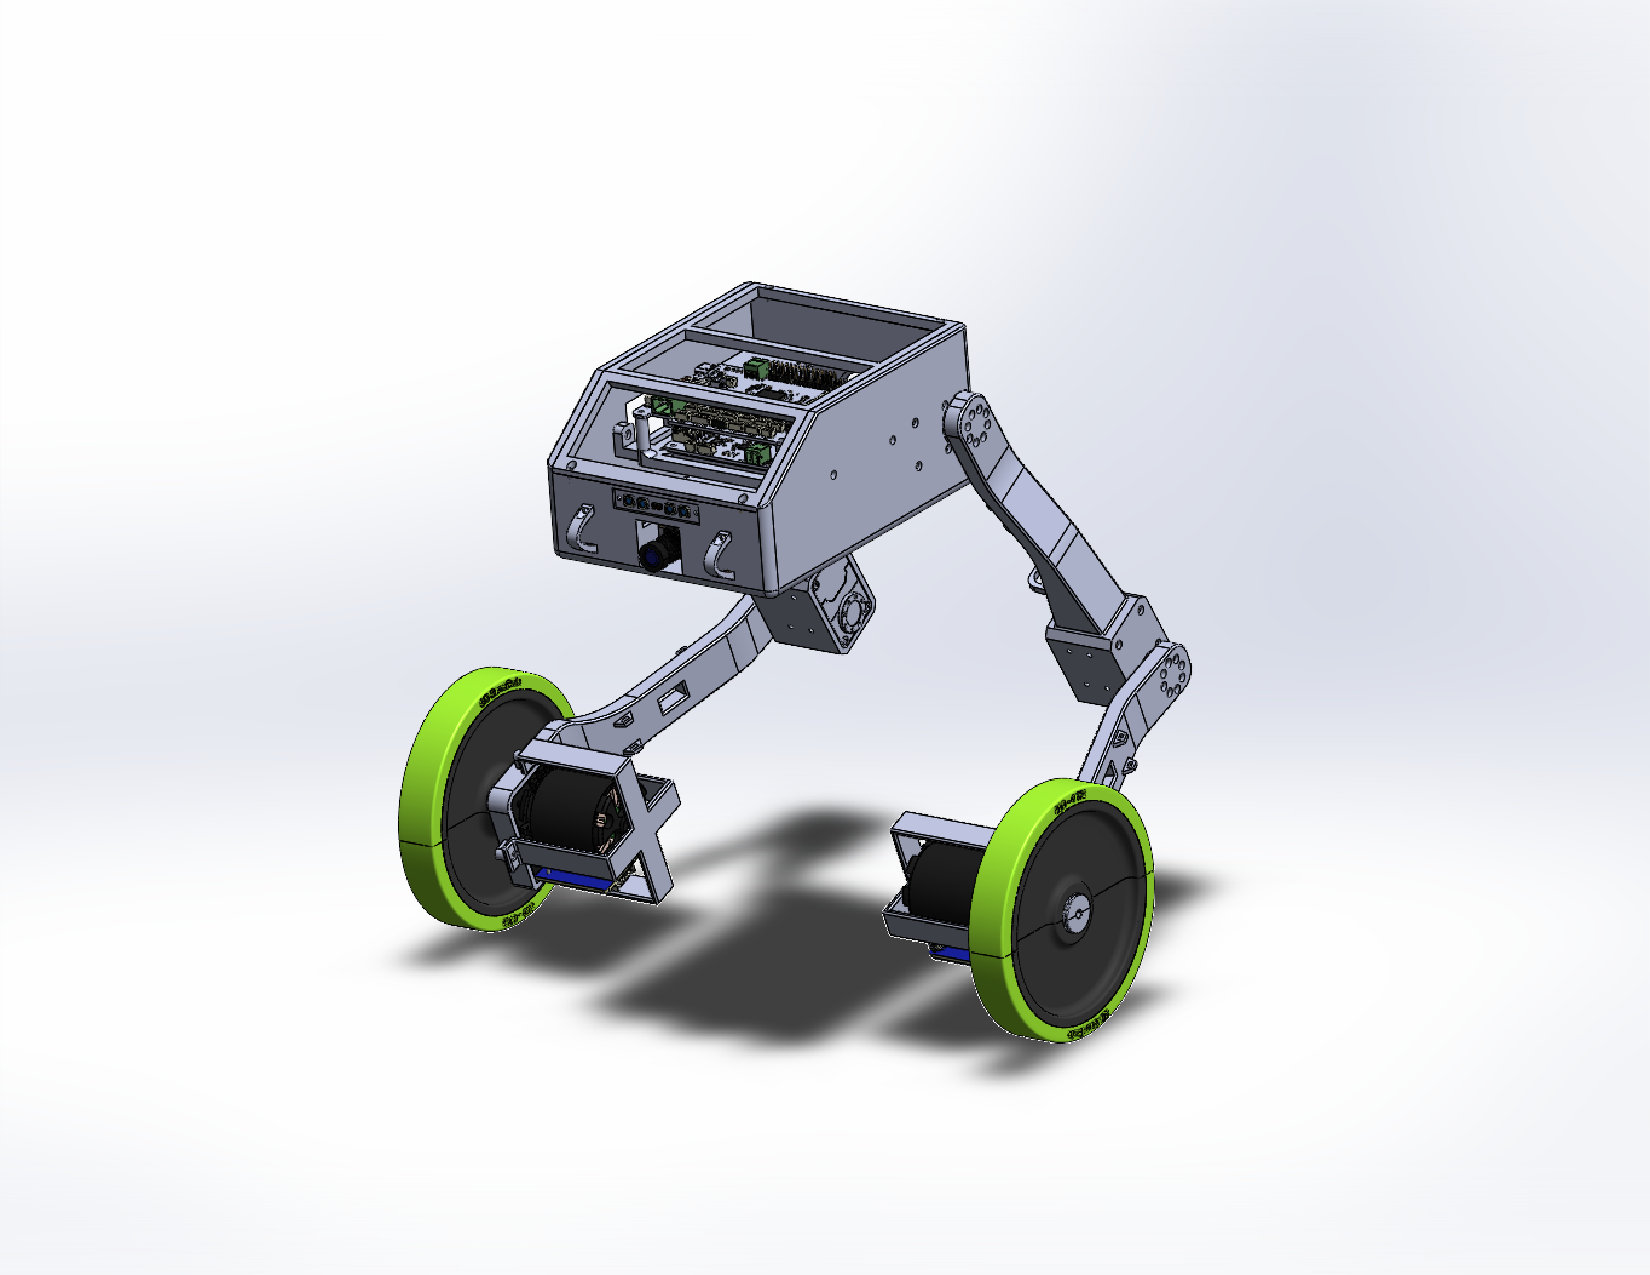
\includegraphics[width=1\textwidth]{Robot_Assembly_V2}
%	\caption[Moment of inertia Schematic representation]{Schematic representation detailing the requisite angles and lengths for calculating the moment of inertia.}
%	\label{fig:Schematic representation detailing the requisite angles and lengths for calculating the moment of inertia.}
%\end{figure}
%\newpage
%\begin{itemize}
%	\item The Robot new design.
%	\item The added degrees of freedom.
%	\item Different motions that can be performed.
%	\item Discussing each component of the robot and things taken into account while designing it.
%	\begin{itemize}
%		\item Body
%		\begin{itemize}
%		\item overall design inspiration
%		\item For the body: the consideration for including all the necessary components in a compact form is to optimize the use of space and at the same time distribute the weight equally.
%		\item The body includes the hip motors, the battery, camera, sensor, a rack that includes the motors drivers board, the micro-controller board attached to the Raspberry Pi.
%		\item fastening features that were specifically designed in order to easily mount the battery, organize the cable between the boards and the rest of the robot parts.
%		\item Features for modular design and easy printing.
%		\end{itemize}
%			\item Thigh
%		\begin{itemize}
%			\item curvature of that joint to give room for the motors
%			\item cable management
%			\item motor cover to insure its fixation.
%		\end{itemize}
%			\item Calf
%		\begin{itemize}
%			\item curvature of that joint and the thigh joint combined make enough room for the wheel motor so the it have clearance from the body.
%			\item cable management
%			\item motor mount and additional frame.
%		\end{itemize}
%	\end{itemize}
%\end{itemize}
\subsection{Leg Design}



\section{Design for Manufacturability and Assembly}
% Discuss how the design facilitates manufacturing and assembly.
% Explain any design choices made to simplify these processes of manufacturing and assembly.
\section{Prototyping and Iterative Design}
% Discuss the process of prototyping.
% Explain how feedback from prototyping phases was incorporated into design revisions.


